\section*{NAIL062 V\&P Logika: 1. sada příkladů}
% po 1. přednášce

\subsection*{Výukové cíle:} Po absolvování cvičení student

    \begin{itemize}\setlength{\itemsep}{0pt}
        \item rozumí pojmům syntaxe výrokové logiky (jazyk, prvovýrok, výrok, strom výroku, podvýrok, teorie), umí je formálně definovat a uvést příklady
        \item rozumí pojmům model, důsledek teorie, umí je formálně definovat a uvést příklady
        \item umí formalizovat daný systém (slovní/výpočetní úlohu, apod.) ve výrokové logice
        \item umí najít modely dané teorie
        \item umí rozhodnout, zda je daný výrok důsledkem dané teorie
        \item má zkušenost s použitím (s pomocí instruktora) tablo metody a rezoluční metody k důkazu vlastností daného systému (např. k řešení slovní úlohy)
    \end{itemize}


\section*{Příklady na cvičení}


\begin{problem}\label{problem:dragons}
    Ztratili jsme se v labyrintu a před námi jsou troje dveře: červené, modré, a zelené. Víme, že za právě jedněmi dveřmi je cesta ven, za ostatními je drak. Na dveřích jsou nápisy:
    \begin{itemize}
        \item Červené dveře: {\it ``Cesta ven je za těmito dveřmi.''}
        \item Modré dveře: {\it ``Cesta ven není za těmito dveřmi.''}
        \item Zelené dveře: {\it ``Cesta ven není za modrými dveřmi.''}
    \end{itemize}
    Víme, že alespoň jeden z nápisů je pravdivý a alespoň jeden je lživý. Kudy vede cesta ven?

    \begin{enumerate}[(a)]
        \item Zvolte vhodný jazyk (množinu prvovýroků) $\mathbb P$.
        \item Formalizujte všechny znalosti jako teorii $T$ v jazyce $\mathbb P$. (Pozor: Axiomy nejsou nápisy na dveřích, ty nemusí být pravdivé.)
        \item Najděte všechny modely teorie $T$.
        \item Formalizujte tvrzení ``Cesta ven je za červenými/modrými/zelenými dveřmi'' jako výroky $\varphi_1,\varphi_2,\varphi_3$ nad $\mathbb P$. Je některý z těchto výroků důsledkem $T$?
        \item Vyzkoušejte si použití tablo metody: Zkonstruujte tablo z teorie $T$ s položkou $F\varphi_i$ v kořeni, budou všechny větve sporné? (Pokuste se vymyslet správné kroky konstrukce tabla, inspirujte se příkladem z přednášky.)
        \item Vyzkoušejte si použití rezoluční metody: Převeďte axiomy teorie $T$, a také výrok $\neg\varphi_i$, do konjunktivní normální formy (CNF). Pokuste se sestrojit rezoluční zamítnutí, zakreslete ho ve formě rezolučního stromu. (Pozor: Nezapomeňte znegovat dokazovaný výrok $\varphi_i$.)
    \end{enumerate}  

    \begin{solution}
        \begin{enumerate}[(a)]
            \item Přirozenou volbou je jazyk $\mathbb P=\{p_1, p_2, p_3\}$, kde $p_i$ znamená `za $i$-tými dveřmi je cesta ven', kde dveře vezměme v pořadí červené, modré, zelené jako v zadání. (Také bychom mohli použít `za $i$-tými dveřmi je drak' nebo `nápis na $i$-tých dveřích je pravdivý'. Důležité je, aby zvolený jazyk byl co nejmenší. Máme-li $p_i$, můžeme např. `za $i$-tými dveřmi je drak' vyjádřit jako `$\neg p_i$', nepotřebujeme další prvovýrok. Dále chceme, aby šlo vlastnosti ze zadání formalizovat co nejsnáze.)
            \item Ze zadání chápeme, že `je drak' znamená totéž, co `není cesta ven'. To, že cesta ven je za právě jedněmi dveřmi, vyjádříme tak, že řekneme, že je za alespoň jedněmi dveřmi, a pro každou dvojici dveří alespoň za jedněmi není:
            $$
            (p_1\lor p_2\lor p_3) \land (\neg p_1\lor\neg p_2) \land  (\neg p_1\lor\neg p_3) \land (\neg p_2\lor\neg p_3)
            $$
            Nyní k nápisům na dveřích, nejprve formalizujeme jejich význam:
            \begin{itemize}
                \item Červené dveře: ``$p_1$''
                \item Modré dveře: ``$\neg p_2$''
                \item Zelené dveře: ``$\neg p_2$''
            \end{itemize}
            Alespoň jeden z těchto nápisů je pravdivý: $p_1\lor \neg p_2\lor\neg p_2$, zjednodušíme na
            $$
            \alpha_2=p_1\lor \neg p_2
            $$
            Podobně to, že alespoň jeden z nápisů je lživý, formalizujeme jako $\neg p_1\lor \neg \neg p_2\lor\neg \neg p_2$, po zjednodušení (rozmyslete si, proč jde o ekvivalentní výrok):
            $$
            \alpha_3=\neg p_1\lor p_2
            $$
            Výsledná teorie je tedy:
            \begin{align*}
                T=\{&\alpha_1,\alpha_2,\alpha_3\}\\=\{&(p_1\lor p_2\lor p_3) \land (\neg p_1\lor\neg p_2) \land  (\neg p_1\lor\neg p_3) \land (\neg p_2\lor\neg p_3), p_1\lor \neg p_2, \neg p_1\lor p_2\}
            \end{align*}
            \item Později se naučíme hledat modely pomocí tablo metody, zatím ale `neefektivní' postup: Nejprve najdeme modely jednoho z axiomů. Protože první axiom je poměrně složitý, možná bude lepší začít axiomem $\alpha_2$. (V principu bychom mohli vyzkoušet postupně všech 8 modelů jazyka $\mathbb P$, a pro každý z nich spočíst pravdivostní hodnotu $\alpha_2$.) Dostáváme:
            $$
            \M_\mathbb P(\alpha_2)=\{(0,0,0),(0,0,1),(1,0,0),(1,0,1),(1,1,0),(1,1,1)\}
            $$
            Nyní zjistíme, ve kterých z těchto modelů platí axiom $\alpha_3$:
            $$
            \M_\mathbb P(\alpha_2,\alpha_3)=\{(0,0,0),(0,0,1),(1,1,0),(1,1,1)\}
            $$
            A nakonec ověříme platnost $\alpha_1$ v každém z těchto 4 modelů:
            $$
            \M_\mathbb P(T)=\M_\mathbb P(\alpha_1,\alpha_2,\alpha_3)=\{(0,0,1)\}
            $$
            \item Při naší volbě jazyka $\mathbb P$ je formalizace jednoduchá: $\varphi_1=p_1$, $\varphi_2=p_2$, $\varphi_3=p_3$. Být důsledkem teorie $T$ znamená platit v každém modelu $T$ (pozor, v každém, ne `v nějakém modelu', to je častá chyba). V našem případě má $T$ jen jeden model, ihned vidíme, že v něm platí $\varphi_3$ a neplatí $\varphi_1$ ani $\varphi_2$. Důsledkem $T$ je tedy z těchto tří jen $\varphi_3$.
            \item Při použití tablo metody postupujeme stejně jako v úvodní kapitole skript (Sekce 1.1.5). Abychom dokázali, že v $T$ platí $\varphi_3$, sestrojíme tablo z teorie $T$, kde do kořene dáme předpoklad $\mathrm{F}p_3$, neboť dokazujeme sporem ($\mathrm{F}$ znamená `False', $\mathrm{T}$ znamená `True'). 
            
            Připomeňme, že tablo rozvíjíme připojováním předpokladů o platnosti axiomů $\mathrm{T}\alpha_i$ ($i\in\{1,2,3\}$) a redukcí položek (připojením příslušných atomických tabel). Pořadí, v jakém to děláme, může značně ovlivnit velikost výsledného tablo důkazu. Dobré je nejprve redukovat položky, jejichž atomická tabla se nevětví, nebo větví, ale některá z větví se ihned stane spornou. Axiomy připojujeme až když jsou potřeba. Často je dobré si rozmyslet, jak bychom v důkazu postupovali my, a podle toho budovat i tablo.

            Všimněte si také, že nedefinujeme atomická tabla pro konjunkce resp. disjunkce tří a více výroků. (Chceme, aby kroky algoritmu byly co nejjednodušší.) Proto např. v $\mathrm{T}p_1\lor p_2\lor p_3$ si nejprve představíme vynechané závorky, $\mathrm{T}p_1\lor (p_2\lor p_3)$, a potom redukujeme ve dvou krocích připojením $\mathrm{T}p_1$ a $\mathrm{T}p_2\lor p_3$:
            
            \begin{center}
                \begin{forest}
                    [$\mathrm{T}p_1\lor (p_2\lor p_3)$
                        [$\mathrm{T}p_1$]
                        [$\mathrm{T}p_2\lor p_3$
                            [$\mathrm{T}p_2$]
                            [$\mathrm{T}p_3$]
                        ]
                    ]            
                \end{forest}
            \end{center}

            (Ještě poznamenáme, že z hlediska tablo metody by bylo trochu lepší mít místo axiomu $\alpha_1$ čtyři samostatné výroky, jichž je konjunkcí. Tím by se konstrukce tabla zkrátila. Algoritmus si ale poradí s jakkoliv složitými axiomy.)

            
            Zde je jeden z možných tablo důkazů ($\oplus$ označuje spornou větev, $\checkmark$ dokončenou bezespornou). Na první pohled může vypadat složitě, ve skutečnosti ale provádíme jednoduchý algoritmus. Rozmyslete si, odkud se vzaly jednotlivé položky, a kde vidíme atomická tabla:
            
            \begin{center}
                \begin{forest}
                    [$\mathrm{F}p_3$
                        [$\mathrm{T}(p_1\lor p_2\lor p_3) \land ((\neg p_1\lor\neg p_2) \land  (\neg p_1\lor\neg p_3) \land (\neg p_2\lor\neg p_3))$
                            [$\mathrm{T}p_1\lor (p_2\lor p_3)$
                                [$\mathrm{T}(\neg p_1\lor\neg p_2) \land  ((\neg p_1\lor\neg p_3) \land (\neg p_2\lor\neg p_3))$
                                    [$\mathrm{T}\neg p_1\lor\neg p_2$
                                        [$\mathrm{T}(\neg p_1\lor\neg p_3) \land (\neg p_2\lor\neg p_3)$
                                            [$\mathrm{T}\neg p_1\lor\neg p_3$
                                                [$\mathrm{T}\neg p_2\lor\neg p_3$
                                                    [$\mathrm{T}p_1\lor \neg p_2$
                                                        [$\mathrm{T}p_1$
                                                            [$\mathrm{T}\neg p_1\lor p_2$
                                                                [$\mathrm{T}\neg p_1$
                                                                    [$\mathrm{F}p_1$, tikz={\node[fit to=tree,label=below:$\otimes$] {};}]
                                                                ]
                                                                [$\mathrm{T}p_2$
                                                                    [$\mathrm{T}\neg p_1$
                                                                        [$\mathrm{F}p_1$, tikz={\node[fit to=tree,label=below:$\otimes$] {};}]
                                                                    ]
                                                                    [$\mathrm{T}\neg p_2$
                                                                        [$\mathrm{F}p_2$, tikz={\node[fit to=tree,label=below:$\otimes$] {};}]
                                                                    ]
                                                                ]
                                                            ]
                                                        ]
                                                        [$\mathrm{T}\neg p_2$
                                                            [$\mathrm{F}p_2$
                                                                [$\mathrm{T}\neg p_1\lor p_2$
                                                                    [$\mathrm{T}\neg p_1$
                                                                        [$\mathrm{F}p_1$
                                                                            [$\mathrm{T}p_1$, tikz={\node[fit to=tree,label=below:$\otimes$] {};}]
                                                                            [$\mathrm{T}p_2\lor p_3$
                                                                                [$\mathrm{T}p_2$, tikz={\node[fit to=tree,label=below:$\otimes$]{};}]
                                                                                [$\mathrm{T}p_3$, tikz={\node[fit to=tree,label=below:$\otimes$]{};}]
                                                                            ]
                                                                        ]
                                                                    ]
                                                                    [$\mathrm{T}p_2$, tikz={\node[fit to=tree,label=below:$\otimes$] {};}]
                                                                ]          
                                                            ]
                                                        ]    
                                                    ]    
                                                ]
                                            ]    
                                        ]
                                    ]
                                ]
                            ]
                        ]
                    ]  
                \end{forest}
            \end{center}
            Co kdybychom zkusili z teorie $T$ dokázat $p_1$, nebo $p_2$? Ukážeme pro $p_1$ (pro $p_2$ si zkuste sami). Do kořene dáme položku $\mathrm{F}p_1$. Postupujeme obdobně, ale alespoň jedna z větví bude i po dokončení (připojení všech axiomů a redukce všech položek) bezesporná. Z bezesporných větví lze potom vyčíst protipříklad (model teorie $T$, ve kterém $p_1$ neplatí).

            Níže je sestrojené dokončené tablo. Ověřte, že jsou použity všechny axiomy a zredukovány všechny položky. Dostáváme dvě dokončené bezesporné větve. Podíváme se na předpoklady o prvovýrocích, které na nich najdeme: Pro obě jsou to $\mathrm{Fp_1}$, $\mathrm{Fp_2}$, $\mathrm{Tp_3}$. To odpovídá modelu $(0,0,1)$, což je opravdu protipříklad: model teorie $T$, ve kterém neplatí $p_1$.

            \begin{center}
                \begin{forest}
                    [$\mathrm{F}p_1$
                        [$\mathrm{T}p_1\lor\neg p_2$
                            [$\mathrm{T}p_1$, tikz={\node[fit to=tree,label=below:$\otimes$] {};}]
                            [$\mathrm{T}\neg p_2$
                                [$\mathrm{F}p_2$
                                    [$\mathrm{T}(p_1\lor p_2\lor p_3) \land ((\neg p_1\lor\neg p_2) \land  (\neg p_1\lor\neg p_3) \land (\neg p_2\lor\neg p_3))$
                                        [$\mathrm{T}p_1\lor (p_2\lor p_3)$
                                            [$\mathrm{T}(\neg p_1\lor\neg p_2) \land  ((\neg p_1\lor\neg p_3) \land (\neg p_2\lor\neg p_3))$
                                                [$\mathrm{T}p_1$, tikz={\node[fit to=tree,label=below:$\otimes$] {};}]
                                                [$\mathrm{T}p_2\lor p_3$
                                                    [$\mathrm{T}p_2$, tikz={\node[fit to=tree,label=below:$\otimes$]{};}]
                                                    [$\mathrm{T}p_3$
                                                        [$\mathrm{T}\neg p_1\lor\neg p_2$
                                                            [$\mathrm{T}(\neg p_1\lor\neg p_3) \land (\neg p_2\lor\neg p_3)$
                                                                [$\mathrm{T}\neg p_1\lor\neg p_3$
                                                                    [$\mathrm{T}\neg p_2\lor\neg p_3$
                                                                        [$\mathrm{T}\neg p_1$
                                                                            [$\mathrm{F}p_1$
                                                                                [$\mathrm{T}\neg p_2$
                                                                                    [$\mathrm{F}p_2$
                                                                                        [$\mathrm{T}\neg p_1\lor p_2$
                                                                                            [$\mathrm{T}\neg p_1$
                                                                                                [$\mathrm{F}p_1$
                                                                                                    [$\mathrm{T}\neg p_1$
                                                                                                        [$\mathrm{F}p_1$, tikz={\node[fit to=tree,label=below:$\checkmark$] {};}]
                                                                                                    ]
                                                                                                    [$\mathrm{T}\neg p_2$
                                                                                                        [$\mathrm{F}p_2$, tikz={\node[fit to=tree,label=below:$\checkmark$] {};}]
                                                                                                    ]
                                                                                                ]
                                                                                            ]
                                                                                            [$\mathrm{T}p_2$, tikz={\node[fit to=tree,label=below:$\otimes$] {};}]
                                                                                        ]
                                                                                    ]
                                                                                ]
                                                                                [$\mathrm{T}\neg p_3$
                                                                                    [$\mathrm{F}p_3$, tikz={\node[fit to=tree,label=below:$\otimes$] {};}]
                                                                                ]
                                                                            ]
                                                                        ]
                                                                        [$\mathrm{T}\neg p_3$
                                                                            [$\mathrm{F}p_3$, tikz={\node[fit to=tree,label=below:$\otimes$] {};}]
                                                                        ]
                                                                    ]
                                                                ]    
                                                            ]
                                                        ]                                                
                                                    ]
                                                ]
                                            ]
                                        ]
                                    ]
                                ]
                            ]
                        ]
                    ]
                \end{forest}
            \end{center}

            \item Při použití rezoluční metody postupujeme stejně jako v úvodní kapitole skript, v Sekci 1.1.6. Abychom dokázali, že v $T$ platí $p_3$, přidáme k teorii $T$ jako axiom výrok $\neg p_3$. Máme tedy $T'=\{\alpha_1,\alpha_2,\alpha_3,\neg p_3\}$. Pomocí ekvivalentních úprav převedeme do CNF (vyjádříme jako konjunkci klauzulí, tj. disjunkcí literálů), v našem případě všechny axiomy už v CNF jsou ($\alpha_1$ je konjunkce tří klauzulí, ostatní jsou klauzulemi). Výsledná CNF formule v množinovém zápisu (pro přehlednost je dobré zapisovat literály v pevném pořadí):
            $$
            S=\{\{p_1,p_2,p_3\},\{\neg p_1,\neg p_2\},\{\neg p_1,\neg p_3\},\{\neg p_2,\neg p_3\},\{p_1,\neg p_2\},\{\neg p_1,p_2\},\{\neg p_3\}\}
            $$
            Nyní sestrojíme rezoluční zamítnutí. Jak vybírat jednotlivé rezoluční kroky? Dobrou heuristikou je fakt, že kratší klauzule obsahuje více informací. Snažíme se tedy začít od nejkratších klauzulí, zde $\{\neg p_3\}$, a sledujeme, kde bychom mohli použít nově odvozené (`naučené') klauzule. Klauzule je často potřeba použít opakovaně. Zde je jedno z možných rezolučních zamítnutí, zakreslené ve formě rezolučního stromu:
            
            \begin{center}
                \begin{forest}
                for tree={grow=north}
                [$ \square $
                    [$ \{\neg p_1\} $
                        [{$ \{\neg p_1, p_2\} $}]
                        [{$ \{\neg p_1,\neg p_2\} $}]
                    ]
                    [$ \{p_1\} $
                        [{$ \{p_1, \neg p_2\} $}]
                        [{$ \{p_1,p_2\} $}
                            [{$ \{p_1,p_2,p_3\} $}]
                            [{$ \{\neg p_3\} $}]
                        ]
                    ]
                ]
                \end{forest}
            \end{center}

            Ověřte, že všechny listy jsou klauzule z $S$ a všechny vnitřní vrcholy vznikly rezolucí ze svých synů. Rezoluční důkaz budeme definovat jako posloupnost klauzulí (kde klauzule jsou buď axiomy, nebo rezolventy předchozích). Takových posloupností odpovídajících našemu stromu je více, zde je jedna z možných:
            $$
            \{\neg p_3\}, \{p_1,p_2,p_3\}, \{p_1,p_2\}, \{p_1, \neg p_2\}, \{p_1\}, \{\neg p_1,\neg p_2\}, \{\neg p_1, p_2\}, \{\neg p_1\}, \square
            $$
        \end{enumerate}
    \end{solution}

\end{problem}


\begin{problem}

    Uvažme \emph{vrcholové pokrytí} (vertex cover) následujícího grafu:    
    \begin{center}
        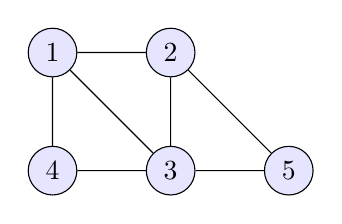
\begin{tikzpicture}[every node/.style={circle,fill=blue!10,draw,minimum size=0.5cm,node distance=1.5cm}]
        \node (1) {$1$};
        \node[right of=1] (2) {$2$};
        \node[below of=2] (3) {$3$};
        \node[left of=3] (4) {$4$};
        \path[draw] (1) -- (2) -- (3) -- (4) -- (1) -- (3);
        \node[right of=3] (5) {$5$};
        \path[draw] (2) -- (5) -- (3);
        \end{tikzpicture}
    \end{center}
    Chceme pro dané $k>0$ zjistit, zda má tento graf nejvýše $k$-prvkové vrcholové pokrytí.

    \begin{enumerate}[(a)]
        \item Zvolte vhodný jazyk (množinu prvovýroků) $\mathbb P$.
        \item Formalizujte ve výrokové logice problém, zda graf na obrázku má nejvýše $k$-prvkové vrcholové pokrytí, pro pevně zvolené $k$. Označme výslednou teorii jako ${VC}_k$.
        \item Ukažte, že ${VC}_2$ nemá žádné modely, tj. graf nemá 2-prvkové vrcholové pokrytí.
        \item Uměli byste k tomu využít tablo metodu? Rozmyslete si postup.
        \item Uměli byste k tomu využít rezoluční metodu? Rozmyslete si postup.
        \item Najděte všechna 3-prvková vrcholová pokrytí.            
    \end{enumerate}

    \begin{solution}
        Vrcholové pokrytí je množina vrcholů $C$ obsahující alespoň jeden vrchol z každé hrany.
        \begin{enumerate}[(a)]
            \item Přirozenou volbou je jeden prvovýrok $p_v$ pro každý vrchol $v\in V$, který popisuje, zda je $v\in C$. Máme tedy $\mathbb P=\{p_v\mid v\in V\}=\{p_1,p_2,p_3,p_4,p_5\}$.
            \item Nejprve formalizujeme, že jde o vrcholové pokrytí (libovolné velikosti). Pro každou hranu $\{u,v\}\in E$ vyjádříme, že $u$ nebo $v$ musí být v $C$. Máme tedy teorii popisující všechna vrcholová pokrytí:
            $$
            VC=\{p_u\lor p_v\mid \{u,v\}\in E, u<v\}
            $$
            
            Zbývá vyjádřit, že platí nejvýše $k$ prvovýroků, což zapíšeme jako disjunkce negací přes všechny $k+1$-prvkové podmnožiny vrcholů:
            $$
            S_{\leq k}=\{\bigvee_{v\in I} \neg p_v\mid I\subseteq V,|I|=k+1\}
            $$
            Výsledná teorie tedy bude $VC_k=VC\cup S_{\leq k}$.
            \item Pro přehlednost zde vypíšeme všechny axiomy teorie $VC_2$ (byť to dělat nemusíme):
            \begin{align*}
                VC_2=&\{p_1\lor p_2,p_1\lor p_3,p_1\lor p_4,p_2\lor p_3,p_2\lor p_5,p_3\lor p_4,p_3\lor p_5,\\
                &\neg p_1\lor\neg p_2\lor\neg p_3,\neg p_1\lor\neg p_2\lor\neg p_4,
                \neg p_1\lor\neg p_2\lor\neg p_5,\neg p_1\lor\neg p_3\lor\neg p_4,
                \neg p_1\lor\neg p_3\lor\neg p_5,\\ &\neg p_1\lor\neg p_4\lor\neg p_5,
                \neg p_2\lor\neg p_3\lor\neg p_4,\neg p_2\lor\neg p_3\lor\neg p_5,
                \neg p_2\lor\neg p_4\lor\neg p_5,\neg p_3\lor\neg p_4\lor\neg p_5\}
            \end{align*}
            Použijeme-li `neefektivní' postup, můžeme si například všimnout, že:
            \begin{align*}
                \M(p_1\lor p_3,p_1\lor p_4,p_3\lor p_4,\neg p_1\lor\neg p_3\lor\neg p_4)&=\{(0,a,1,1,b),(1,a,0,1,b),(1,a,1,0,b)\mid a,b\in\{0,1\}\}\\
                \M(p_2\lor p_3,p_2\lor p_5,p_3\lor p_5,\neg p_2\lor\neg p_3\lor\neg p_5)&=\{(a,0,1,b,1),(a,1,0,b,1),(a,1,1,b,0)\mid a,b\in\{0,1\}\}\\
            \end{align*}
            Jde o 2-prvková vrcholová pokrytí podgrafů $\{1,3,4\}$ a $\{2,3,5\}$. Průnik těchto množin je
            $$
                \{(0,0,1,1,1),(0,1,1,1,0),(1,1,0,1,1),(1,0,1,0,1),(1,1,1,0,0)\}
            $$
            Žádný z těchto modelů ale nesplňuje ostatní axiomy, např. v prvním neplatí $\neg p_3\lor\neg p_4\lor\neg p_5$.
            \item Tablo metodu použijeme k důkazu, že v teorii $VC_2$ platí spor, tj. výrok $p_1\land \neg p_1$. Ten vložíme do kořene s příznakem $\mathrm{F}$ (`False'), tj. dokazujeme spor, sporem. Ukážeme jen část konstrukce (levou větev).
           
            \begin{center}
                \begin{forest}
                    [$\mathrm{F}p_1\land\neg p_1$
                        [$\mathrm{F}p_1$
                            [$\mathrm{T}p_1\lor p_2$
                                [$\mathrm{T}p_1$, tikz={\node[fit to=tree,label=below:$\otimes$] {};}]
                                [$\mathrm{T}p_2$
                                    [$\mathrm{T}p_1\lor p_3$
                                        [$\mathrm{T}p_1$, tikz={\node[fit to=tree,label=below:$\otimes$] {};}]
                                        [$\mathrm{T}p_3$
                                            [$\mathrm{T}p_1\lor p_4$
                                                [$\mathrm{T}p_1$, tikz={\node[fit to=tree,label=below:$\otimes$] {};}]
                                                [$\mathrm{T}p_4$
                                                    [$\mathrm{T}\neg p_2\lor (\neg p_3\lor \neg p_4)$
                                                        [$\mathrm{T}\neg p_2$
                                                            [$\mathrm{F}p_2$, tikz={\node[fit to=tree,label=below:$\otimes$] {};}]
                                                        ]
                                                        [$\mathrm{T}\neg p_3\lor \neg p_4$
                                                            [$\mathrm{T}\neg p_3$
                                                                [$\mathrm{F}p_3$, tikz={\node[fit to=tree,label=below:$\otimes$] {};}]
                                                            ]
                                                            [$\mathrm{T}\neg p_4$
                                                                [$\mathrm{F}p_4$, tikz={\node[fit to=tree,label=below:$\otimes$] {};}]
                                                            ]
                                                        ]
                                                    ]
                                                ]
                                            ]
                                        ]
                                    ]
                                ]
                            ]
                        ]
                        [$\mathrm{F}\neg p_1$
                            [$\mathrm{T}p_1$, tikz={\node[fit to=tree,label=below:$\vdots$] {};}
                            ]
                        ]
                    ]
                \end{forest}
            \end{center}

            (Alternativně bychom mohli použít tablo metodu adaptovanou přímo na hledání modelů, do kořene dát platnost prvního axiomu, a rozvíjet tablo za přidávání předpokladů platnosti ostatních axiomů: každý model musí souhlasit s některou větví, všechny nám ale vyjdou sporné.)
            
            \item Všechny axiomy už jsou v CNF. Stačí najít rezoluční zamítnutí teorie $VC_2$ (tedy rezoluční důkaz prázdné klauzule $\square$), z toho plyne, že $VC_2$ nemůže mít model. Nakreslíme jen (jeden možný) rezoluční strom:
            
            \begin{center}
                \scalebox{0.8}{
                \begin{forest}
                    for tree={grow=north}
                    [$ \square $
                        [$ \{\neg p_1\} $
                            [{$ \{p_2\} $}
                                [{$ \{p_2,\neg p_3\} $}
                                    [{$ \{p_1,p_2\} $}]
                                    [{$ \{\neg p_1,p_2,\neg p_3\} $}
                                        [{$ \{p_2,p_5\} $}]
                                        [{$ \{\neg p_1,\neg p_3,\neg p_5\} $}]
                                    ]
                                ]
                                [{$ \{p_2,p_3\} $}]
                            ]
                            [{$ \{\neg p_1,\neg p_2\} $}
                                [{$ \{p_3\} $}
                                    [{$ \{\neg p_2, p_3\} $}
                                        [{$ \{p_1,p_3\} $}]
                                        [{$ \{\neg p_1,\neg p_2, p_3\} $}
                                            [{$ \{p_3,p_5\} $}]
                                            [{$ \{\neg p_1,\neg p_2,\neg p_5\} $}]
                                        ]
                                    ]
                                    [{$ \{p_2,p_3\} $}]
                                ]    
                                [{$ \{\neg p_1,\neg p_2,\neg p_3\} $}]
                            ]
                        ]
                        [$ \{p_1\} $
                            [{$ \{p_1,\neg p_2\} $}
                                [{$ \{p_1,p_3\} $}]
                                [{$ \{p_1,\neg p_2,\neg p_3\} $}
                                    [{$ \{p_1,p_4\} $}]
                                    [{$ \{\neg p_2,\neg p_3,\neg p_4\} $}]
                                ]
                            ]
                            [{$ \{p_1,p_2\} $}]
                        ]
                    ]
                \end{forest}
                }
            \end{center}
            

            \item Zde uveďme jen správnou odpověď: $\M(VC_3)=\{(0,1,1,1,0),(1,0,1,0,1),(1,1,1,0,0)\}$ což odpovídá množinám vrcholů $\{2,3,4\},\{1,3,5\},\{1,2,3\}$. Použití tablo metody by bylo trochu pracnější, můžete si ale zkusit dokázat (tablo metodou nebo rezolucí), že v pokrytí musí vždy být vrchol 3.
        \end{enumerate}
    \end{solution}

\end{problem}


\section*{Další příklady k procvičení}


\begin{problem}
    
    Uvažme následující tvrzení:
    \begin{enumerate}[(i)]
        \item {\it Ten, kdo je dobrý běžec a má dobrou kondici, uběhne maraton.}
        \item {\it Ten, kdo nemá štěstí a nemá dobrou kondici, neuběhne maraton.}
        \item {\it Ten, kdo uběhne maraton, je dobrý běžec.}
        \item {\it Budu-li mít štěstí, uběhnu maraton.}
        \item {\it Mám dobrou kondici.}
    \end{enumerate}
    Podobně jako v prvním příkladu popište situaci pomocí výrokové logiky:
    \begin{enumerate}[(a)]
        \item Formalizujte tato tvrzení jako teorii $T$ nad vhodnou množinou prvovýroků.
        \item Najděte všechny modely teorie $T$. 
        \item Pokuste se využít k hledání modelů také \emph{tablo metodu}.
        \item Napište několik různých důsledků teorie $T$.
        \item Najděte CNF teorii ekvivalentní teorii $T$.
    \end{enumerate}
    
\end{problem}


\begin{problem}

    Mějme tři bratry, každý z nich buď vždy říká pravdu anebo vždy lže.
    \begin{enumerate}[(i)]
        \item Nejstarší říká: \emph{``Oba mí bratři jsou lháři.''}
        \item Prostřední říká: \emph{``Nejmladší je lhář.''}
        \item Nejmladší říká: \emph{``Nejstarší je lhář.''}
    \end{enumerate}
    Pomocí výrokové logiky ukažte, že nejmladší bratr je pravdomluvný.
     
\end{problem}


\begin{problem}
    Mějme pevně dané Sudoku. Popište, jak vytvořit teorii (ve výrokové logice), jejíž modely jednoznačně odpovídají validním řešením.
\end{problem}


\begin{problem}

    Formalizujte následující tvrzení ve výrokové logice:
    \begin{enumerate}[(a)]\it
        % \item Borůvky podél cesty jsou zralé, ale králíčci v oblasti nebyli pozorováni.

        \item Králíčci v oblasti nebyli pozorováni a procházení po cestě je bezpečné, ale borůvky podél cesty jsou zralé.
        
        \item Pokud jsou borůvky podél cesty zralé, pak je procházení po cestě bezpečné pouze tehdy, pokud králíčci nebyli v oblasti pozorováni.
        
        \item Procházet se podél cesty není bezpečné, ale v oblasti nebyli pozorováni králíčci a borůvky podél cesty jsou zralé.
        
        \item Aby bylo procházení po cestě bezpečné, je nezbytné, ale nedostačující, aby borůvky podél cesty nebyly zralé a králíčci nebyli v oblasti pozorováni.
        
        \item Procházení po cestě není bezpečné, kdykoli jsou borůvky podél cesty jsou zralé a v oblasti byli pozorováni králíčci.
    
    \end{enumerate}
    
\end{problem}





\begin{problem}

    Formalizujte následující vlastnosti matematických objektů ve výrokové logice:
    \begin{enumerate}[(a)]
        % \item Pro pevně daný (konečný) graf $G$, že je regulární stupně 3.
        \item Pro pevně daný (konečný) graf $G$, že má perfektní párování.
        \item Pro pevně danou částečně uspořádanou množinu, že je totálně (lineárně) uspořádaná.
        \item Pro pevně danou částečně uspořádanou množinu, že má nejmenší prvek.
    \end{enumerate}

\end{problem}


\begin{problem} 
    
    Pro následující výroky nakreslete strom výroku, a najděte množinu modelů: \\(a) $(p \to q) \leftrightarrow \neg (p \wedge \neg q)$\qquad (b) $(p \leftrightarrow q) \leftrightarrow ((p \vee q) \to (p \wedge q))$

\end{problem}




\section*{K zamyšlení}


\begin{problem}

    Připomeňte si definici \emph{stromu výroku}.
    \begin{enumerate}[(a)]
        \item Dokažte podrobně, že každý výrok má jednoznačně určený strom.
        \item Platilo by to, i kdybychom v definici výroku nahradili symboly %pro levou a pravou závorku 
        `(', `)' symbolem `|'?
        \item Co by se stalo, pokud bychom závorky vůbec nepsali?
    \end{enumerate}

\end{problem}


% \begin{problem}

%     Připomeňte si definici \emph{výroku}. Jaké jsou možné délky výroků, tj. pro jaká $n\in\mathbb N$ existuje výrok délky právě $n$? (Uvažujte konečný jazyk, každý prvovýrok je jen jeden symbol. Výrok obsahuje všechny závorky dané definicí, konvence o vynechávání závorek se týká jen toho, jak výrok zapisujeme my.)

% \end{problem}
